\section{Introduction}
\subsection{Introduction} 
Phil Beadle \cite{website:TES} explains in his article why the seating plan is the single most important piece of behavioural modification equipment in a teachers toolbox. Phil lays more emphasis on how the way pupils sit in the classroom impacts their learning and their participation in the classroom. A survey of students asking them ``How do they learn best?'' made it clear that students learn best in groups, as they all replied they work better in groups.
\subsection{The Problem}
Teachers have a wide range of tools and software applications to aide them with their daily tasks and most of these software suites come with a classroom seating feature but these tools are developed with a one size fits all ideology.There is research that lays out how best to group students in a classroom but since almost all the tools teachers have at their disposal are rigid with no flexibility they cannot experiment with these research findings to the better of their students.

Teachers are known to take matters in their hands by performing seating arrangements on a piece of paper or worse not bother with the extra work but go with the default structure to the detriment of the students.

\subsection{The Solution}
A better way to solve this and to encourage teachers to experiment with proven findings on how to get the best out of students in a classroom would be to develop a web application that helps them with seating arrangements and one with an \emph{Adaptive User Interface} and breaks away from the one size fits all ideology to a one size fits none ideology. Where the interface can make implicit inference on how the system is being used and how best to help the user complete their tasks.

\subsection{Main Concepts}
The notion of Adaptive User Interfaces has been around for several years, gathering an enormous amount of interest in the research community. Over the years a lot of technological advancements have been made in addition to standards and techniques to achieve adaptiveness on the user facing or interface layer of software applications. Example [interbook@Aha]. \cite{brusilovsky2007user} 

An adaptive user interface monitors the users activity trying to identify usage patterns and automatically adjust the interface components or content provided by the system to accommodate such user differences as well as changes in user skills, knowledge and preferences.\cite{alvarez2007current}

This can be achieved through a number of approaches; namely Task models, User Models and Artificial Intelligence Techniques. This project utilises User Model Technique. 

User models are used to generate or adapt user interfaces at runtime, to address particular user needs and preferences. User models are also known as user profiles, personas or archetypes. The user preferences and needs are represented by variables \cite{W3C}.
\subsection{Project Aims}
This project aims to use the User Model approach to develop a web application with an \emph{Adaptive User Interface} that teachers can use to manage their classrooms in terms of seating pairing and arrangement of pupils. The underlying User Model of the application is based on research findings on how to best group students in a classroom:

\begin{itemize}
    \item Groups - A general rule that applies to the application domain (seating plan); students work better in groups.
    \item Boys and Girls together - A general rule of pairing boys and girls together ; boys work better when paired with girls with a slightly lower ability. \cite{OFSTED}
    \item Current Context - that is, the current highly rated seating pattern by the teacher. 
\end{itemize}

The figure below \ref{fig:User-Model} illustrates the overview of the system and what it does. Teachers import student data in a Comma Separated Values format this forms part of the teachers user data. If the teacher is a returning user then any previously used seating plan rated highly by the user forms part of his or her user data. if the user is new then this variable is populated with the default which obeys the first two of the rules mentioned in the previous paragraph.

The adaptation effect is achieved by implicitly identifying patterns in the seating plans favoured by the user( highly rated previously used plans), although the system requires the user to explicitly score the plans they use based on its effectiveness and how the students responded. The User Model algorithm alters its rules based on these patterns. Example a teacher despite the research indicating boys work best with slightly lower ability girls may have his or her most effective seating plan being one where boys are paired together with other boys. The UM algorithm would identify this and then change its rules to reflect this, that is to reflect the teachers preferences.

The adaptation rule is initially applied when the teacher uses the system for the first time, the default rule is applied this time as the system does not have any history of seating plans to work with. The effect is evident when the user moves a student around in the classroom space, if a pairing is the best as specified by the current rule they are highlighted green and if it is the worse they are highlighted red. These adaptations are in the form of recommendations - the user does not necessarily have to follow this, they can override and form their own seating rules by telling the system how effective their rules ( seating pairing) are.


\begin{figure}[!ht]
\caption{User Modeling Overview}
    \label{fig:User-Model}
    \centering
    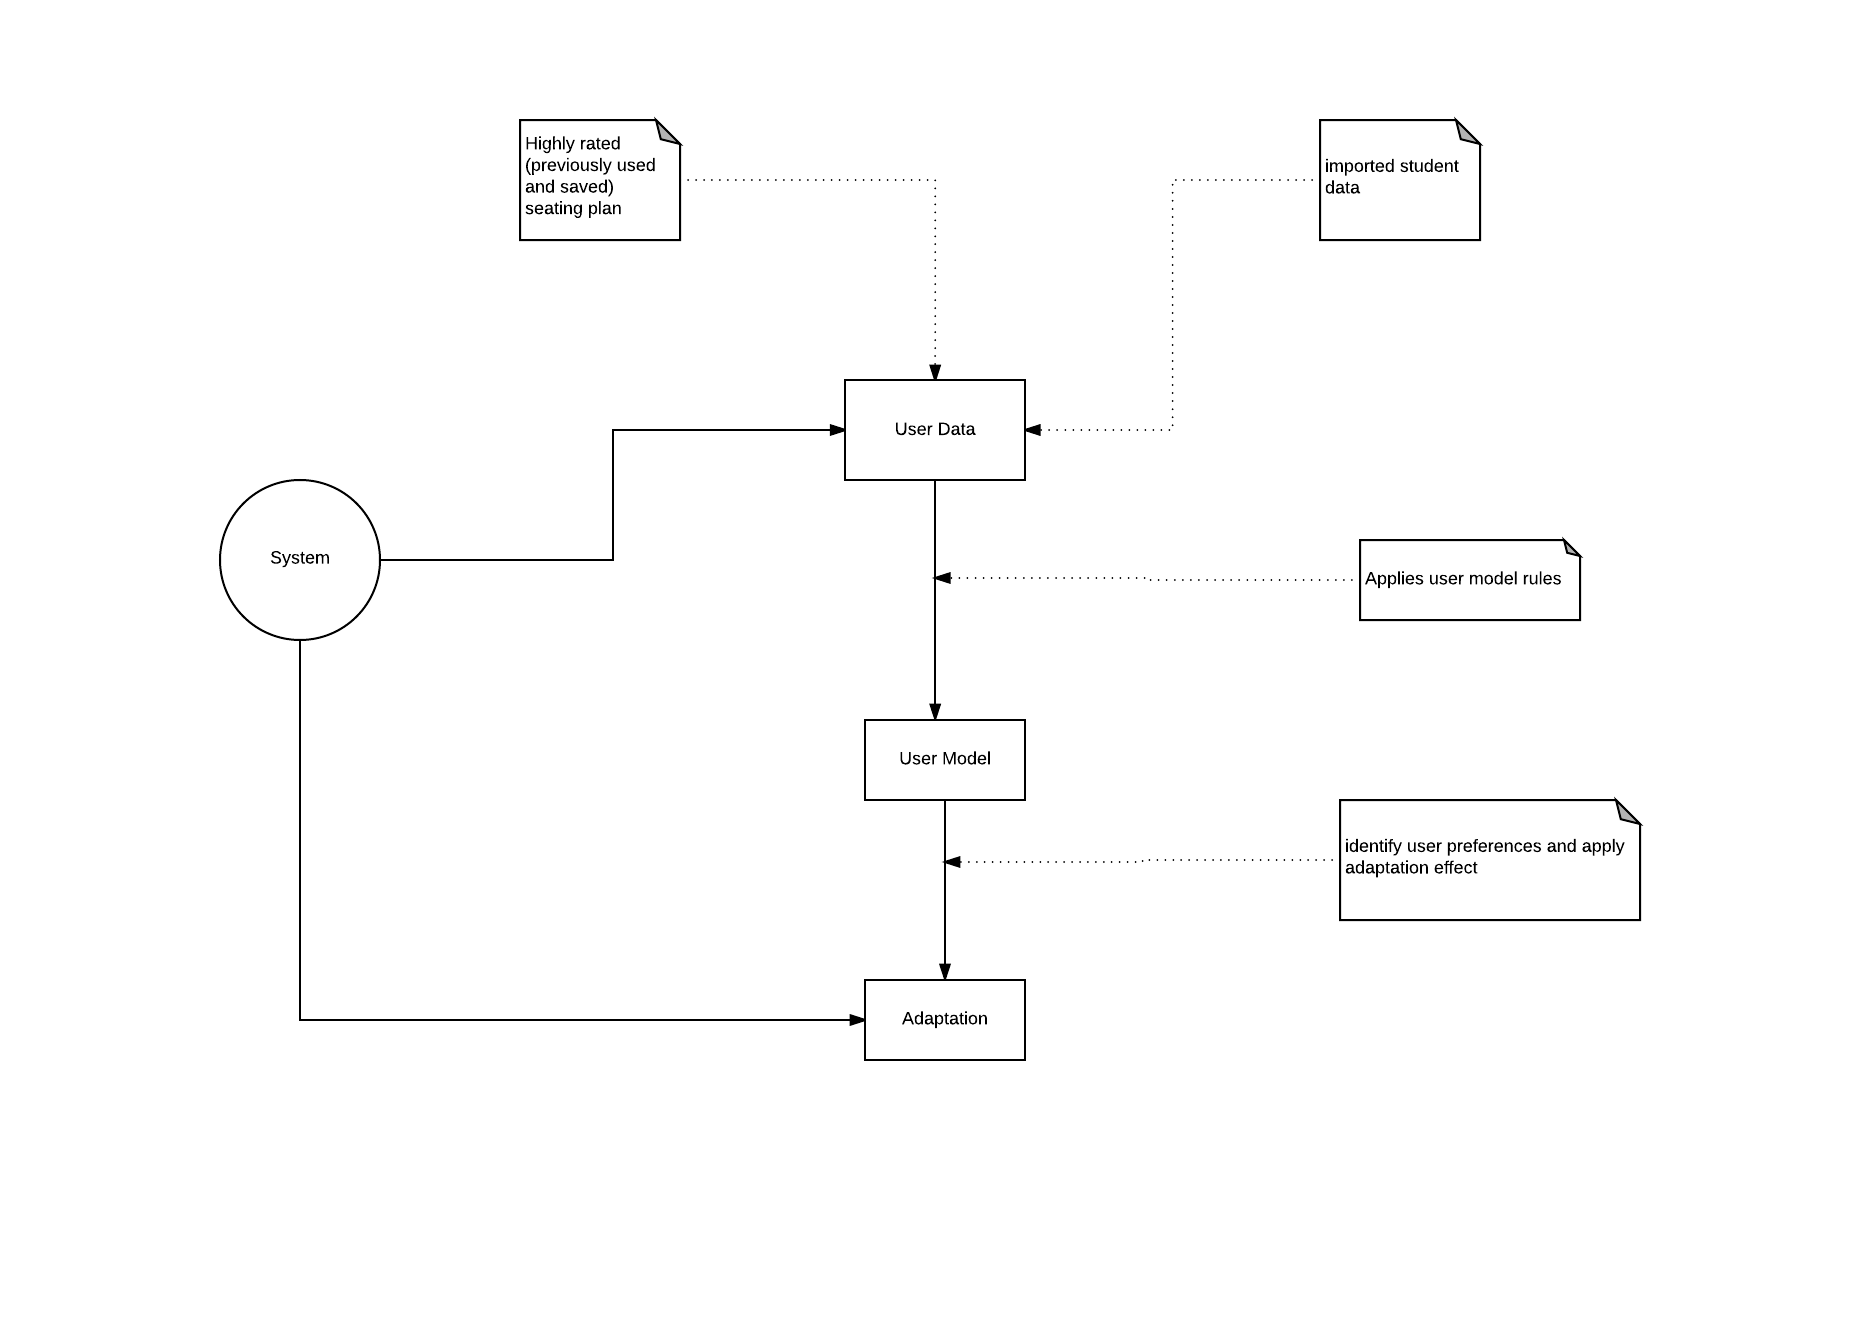
\includegraphics[scale=0.5]{figures/UM_Overview}
\end{figure}

The main components of the system are classroom space( canvas ) on which students are rendered, a history stack (holding references) to all seating plans used by the user and a User Model algorithm that identify usage patterns and apply adaptation rules respectively. We will discuss the implementation and design in detail in the next chapters.

\subsection{Paper Structure}
In chapter two of this paper we will discuss existing approaches to classroom management or behavioural tools, the theories behind classroom management or seating arrangements and  critically discuss existing classroom management tools and or systems under literature review.

Chapter 3 looks at the design requirements of the system in detail, discussing the non-functional and functional requirements as well as user requirements of the system.

We will talk about the implementation of the overall system and the architecture as well as design patterns adopted in chapter 4. We will discuss the User Model algorithm in detail as well as show some code snippets of relevant methods that play a critical part in providing the user with the right adaptation effect.

In chapter 5 we will discuss the testing and evaluation techniques used throughout the project and critical discuss components of the system that passed or failed and why they failed the testing process.

We conclude in chapter 6 by discussing what the project has been able to achieve, what could be done to extend or improve on what has been done so far in terms of future work and the importance of the result of the project to the teaching profession and students as a whole.

